%
%  $Description: Author guidelines and sample document in LaTeX 2.09$
%
%  $Author: mankit $
%  $Date: 2008/05/20 07:24:15 $
%  $Revision: 1.41 $
%

\documentclass[times, 10pt,twocolumn]{article}
\usepackage{latex8}
\usepackage{times}
\usepackage{amssymb}
\usepackage{amsmath}
\usepackage{stmaryrd}
\usepackage{graphicx}
\usepackage{fancyvrb}
\usepackage{color}
\usepackage[small]{caption}
%\documentstyle[times,art10,twocolumn,lat ex8]{article}

%-------------------------------------------------------------------------
% take the % away on next line to produce the final camera-ready version
%\pagestyle{empty}

%-------------------------------------------------------------------------
\begin{document}

  \title{Side Channel Elimination on a Precision Timed Architecture}

  \author{Isaac Liu, David McGrogan \\
    Center for Hybrid and Embedded Software Systems, EECS \\
    University of California, Berkeley \\
    Berkeley, CA 94720, USA \\
    \{\tt liuisaac, dpmcgrog\}@eecs.berkeley.edu
  }


\maketitle
\thispagestyle{empty}

\begin{abstract}
Eliminating side channel attacks for encryptions
\end{abstract}

%encryption info
%	explain a little about the applications of encryption and how it works
%- side channel attack info
%	brief summary on side channel attacks, including timing, cache, branch predictor (i can add this in later), and maybe even power
%- Pret
%	Explanation of the architecture, and deadline instruction (you can take some graphics off our paper or the current poster template)
%-source code
%	I'll add in some source code snap shots of how to program with deadlines
%-Results
%	Plots of data and timing information

\section{Outline and Breakdown}
\begin{itemize}
\item abstract, Introduction  - Isaac
\item Related Work - David
\item Encryption and Side Channel Attacks - David
\item PRET  - Isaac 
\item Results  - Isaac
\item Conclusion and future work - David
\end{itemize}

%------------------------------------------------------------------------------
\section{Introduction}
In order for a secure software to be truly secure, its underlying hardware must also be secure. In other words, the underlying hardware must not emit any information regarding the secure process that's executing on the hardware. 

Kelsey et al.~\cite{Kelsey98sidechannel} introduce the idea of side-channel cryptanalysis, which is cryptanalysis using implementation data. 

Computer architects have made amazing advancements in architecture design to allow for faster processing. The introduction and improvement of pipelines, branch predictors and caches allow for better speculative execution. Hardware threading mechanisms such as simultaneous multi-threading improve the utilization and throughput of the processor. However, these improvements come at a cost. Because these mechanisms improve performance by speculatively executing instructions, the complexity required to maintain state and recovery is enormous. Programs executed on modern processors now have improved average case performance, but unpredictable and non-repeatable execution times. Edwards and Lee\cite{edwards2007case} argued, for the purpose of Real Time Systems, that we needed to reconsider the importance of predictability and repeatability in the core design of the architecture. We argue that this reconsideration is also needed for security systems, because secure software is only as secure as its underlying execution platform. 


\section{Related work}

\section{Background}
% 1 - 1.5 page
\textcolor{red}{David, make sure to mention some proposed solutions for each one. I mention in the next paragraph that these individual solutions mentioned in this paragraph are helpful, but they don't tackle the root cause.}

\subsection{Encryption}
The goal of encryption is to make information illegible to anyone without special knowledge, generally expressed as a key.  It is naturally of tremendous worth in the Information Age, especially to entities such as governments and businesses, which have known adversaries.  Encryption algorithms generally use a so-called trapdoor function, which is easy to compute in one direction but difficult (according to current knowledge) to compute in the other direction without an additional piece of information.  These functions are based on operations such as prime factorization or taking discrete logarithms; as years of concerted effort has failed to produce an efficient algorithm to invert them, the cryptographic algorithms founded on them are used with a large amount of confidence in the algorithms' security.  That is, given all details of the encryption algorithm except for the key, an adversary will not be able to read the encoded information with any reasonable amount of computational power.  [image: traditional model of cryptography]
\subsection{Side Channel Attacks}
Traditional attacks on cryptographic algorithms use only the input and output of the algorithm, treating it like a monolithic black box.  In contrast, side channel attacks circumvent the mathematical complexity of reversing encryption by getting additional data about the encryption process.  [image: model with info. leakage]  Depending on the algorithm and its implementation, a wide variety of information leaks may exist on a number of different physical channels.  The attacks which exploit these channels differ greatly in the difficulty of implementation (or the information is easier or harder to get), ranging from simple in the case of timing attacks to requiring physical access in the case of power attacks.
\subsubsection{Timing attacks}
Timing attacks observe variation in the time spent by an encryption algorithm, often with a known input, and use this information to deduce the key.  This timing data are often compared to a duplicate of the encrypting hardware belonging to the attacker over various keys, enabling better feedback.  Vulnerability to this attack depends on the software implementation of the algorithm, but is rather widespread due to the general drive toward fast algorithms.
\subsubsection{Caching attacks}
Caching attacks use a spy thread running concurrently with the encryption program on the target hardware.  The spy thread occupies all lines in the cache, and detects the loading of data from different locations in memory by timing the return of the data; if the encrypting program has evicted the soy thread's data for its own use, the spy thread's load operation will take longer.  For some algorithms, such as AES, this enables information about the key (which has precomputed components) to be obtained.
\subsubsection{Branch Predictor attacks}
Similar to caching attacks, branch predictor attacks involve a spy program running concurrently with the encryption program.  In this case, the spy thread fills all entries in the branch predictor table with a known value and constantly checks up on those values.  By counting the cycles required for a branch, the spy program detects any change in the state of the branch predictor and therefore infers the control flow of the encryption thread, revealing information about the key.
\subsubsection{Power attacks}
Power attacks use the changing power consumption of the processor to infer the activity of the encryption software over time.  Differences in algorithm activity based on the key will be revealed by the fluctuations they create in processor energy use.  Power attacks require measurement of the power intake of the processor, and are thus generally impossible without physical access to the target hardware, but this is no obstacle in cases such as consumer electronics.

\section{Elimination of Side Channel Attacks}
We can see a pattern in all of the side channel attacks that are mentioned above. The attacker collects information from the implementation on the underlying hardware, and use it to infer information regarding the encryption algorithm, which can lead to exposure of the secret key. The branch predictor side channel attack and cache side channel attack both attack a single shared resource from the hardware. By writing a spy process to hog up that resource, you can easily monitor another thread's access to the same resource and therefore monitor the activity of the thread. The timing side channel attack attacks the algorithm's uncontrollable execution time on the processor, and predicts the execution flow to obtain the encryption key. Several individual methods have been proposed for to counter the attacks, but they don't tackle the principle cause of the vulnerability -- the uncontrollable and unpredictable execution of software on modern computer architectures. Lickly and Liu~\cite{pret_cases08} introduced PRET (PREcision Timed Architecture), an architecture that delivers predictable timing along with predictable function and performance. This architecture tackles the root cause of side channel attacks by design, eliminating the vulnerability.

\begin{figure}[ht]
  \centering
  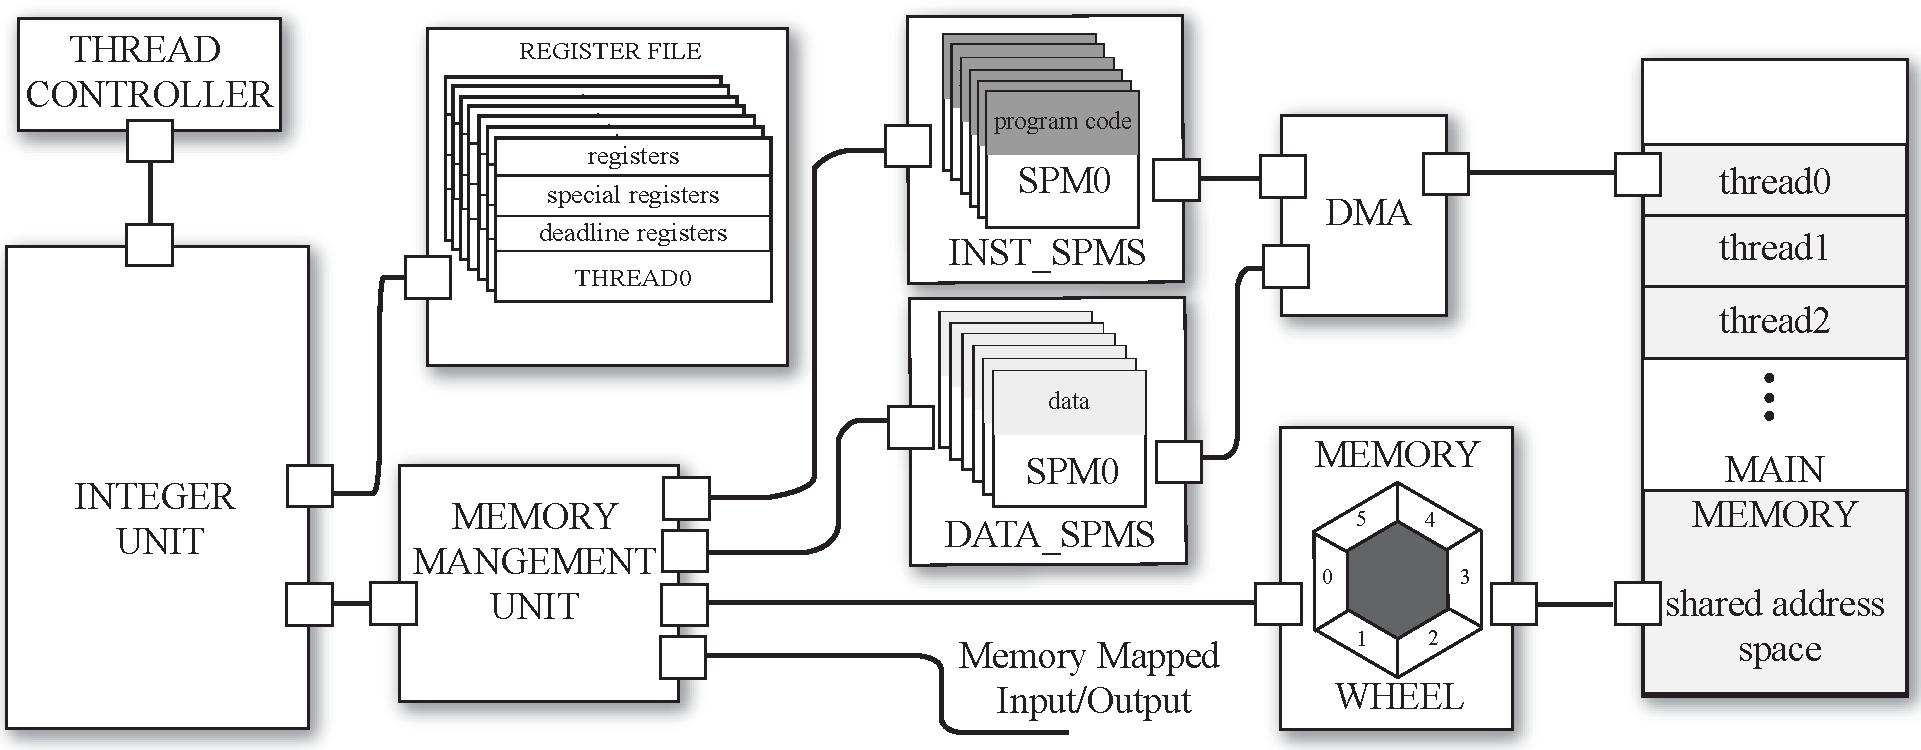
\includegraphics[scale=.25]{./images/top_arch.pdf}
  \caption{Block Diagram of PRET Architecture}
  \label{fig:top_arch}
\end{figure}

We present an overview of the PRET architecture in the context of eliminating side channels attacks, and refer interested users to ~\cite{pret_cases08} for more details. We assume the reader has a basic understanding of computer architectures, such as how pipelining and caches work. Readers that aren't familiar with these terms are advised to see \cite{patterson2005coa} for an introduction.
%\begin{wrapfigure}{r}{0pt}
%  \end{wrapfigure}
\subsection{PRET Architecture}
A block level diagram of the PRET architecture is shown in figure~\ref{fig:top_arch}. The core integer pipeline unit of the PRET architecture implements a thread-interleaved pipelined. Hardware units that keep the processor's state such as register files or local on chip memories are duplicated for each hardware thread. Threads are scheduled to execute in a predictable round-robin fashion. Scratchpad memories\cite{Banakar2002}(SPM) are employed instead of caches to allow controlled and predictable access to local on chip memories. A memory controller facilitates time triggered access to the off-chip main memory through a memory wheel to decouple the access to memory of each thread from another. In addition, ISA support is provided to bring timing semantics to the software level.

\subsubsection {Thread-Interleaved Pipeline}
Pipeline hazards occur because the next instruction to be fed into the pipeline does not have the required information to be executed. Conditional branches are the prime example -- the pipeline cannot fetch and execute the next instruction without knowing what it is. The penalty of hazards can be mitigated by introducing hardware units that speculate the next state. Branch predictors speculate the next instruction. Caches speculate the data that will be accessed in the near future. If the speculation is correct, there is no penalty. But if it is incorrect, then the processor must work extra to recover by discarding the speculated work and re-executing the correct procedure. These mechanisms are the main cause of unpredictable execution time because in software there is no way of knowing whether the hardware speculation is correct or not. 

However, if we can remove pipelining hazards, then we can remove the need for the speculation units. Lee~\cite{lee1987pipeline1} proposed using thread interleaved pipeline to remove data dependencies and control hazards in the pipeline to get predictable and repeatable behavior. The basic idea is shown in figure \ref{fig:int_pipe}. 
\begin{figure}[ht]
  \centering
  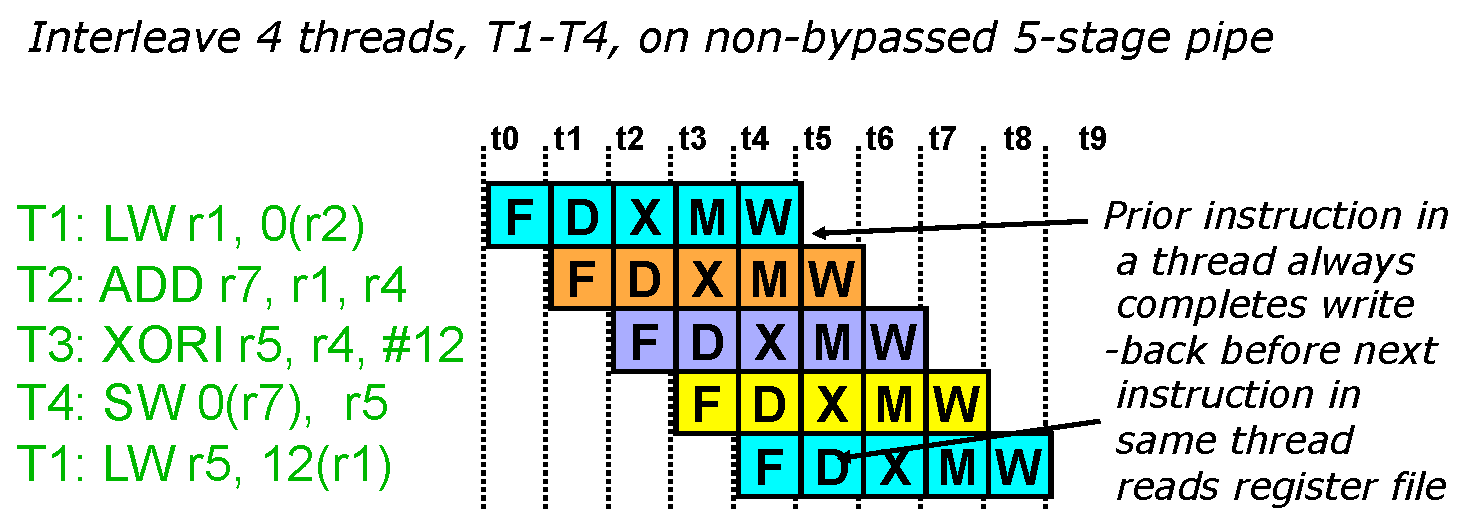
\includegraphics[scale=.35]{./images/interleavedpipeline.pdf}
  \caption{How interleaved threading removes data dependencies}
  \label{fig:int_pipe}
\end{figure}

By thread-interleaving, we can completely remove any data forwarding logic in the processor, along with the branch predictors, because we have no need to try and speculate the next instruction that needs to be executed. Simply by focusing on repeatable and predictable behavior in the design of the pipeline, we removed the vulnerability that caused the branch predictor attack. 

\subsubsection {Memory System}
Fast access on-chip memories is a requirement for modern processors. The the high clock speed of the processor combined with the long latency it takes to access main memory results in hundreds of cycles lost when the processor needs to access the off-chip main memory. Caches are hardware controlled fast access memories that speculate and pre-fetch the data from main memory based on temporal and spatial locality. If the cache control speculation is accurate, then access to data can complete in one cycle of the processor. However, if mis-predicts occur, the time it takes to access the data is drastically longer. Thus, cache hits and misses often determine the performance of a system, resulting in a major source of timing unpredictability~\cite{thiele:04:predictable}.

Unlike the branch predictor, removing fast access memories in not an option, since it will result in a huge performance overhead. Instead, we use scratchpad memories as an alternative to caches. Scratchpad memory brings the control over the fast access memory to software. The compiler can pre-allocate the data locations in the fast access memory, resulting in predictable performance (since we always know which accesses are hits or misses). The software may also control the loading of scratchpad memories at run time by using Direct Memory Access instructions without a lost of predictability. Ongoing research have shown methods to efficiently manage the scratchpads~\cite{avissar2002oma, Bandyopadhyay:EECS-2006-105, Patel:EECS-2008-115} to optimize the performance of program, but is beyond the scope of this paper. 

Because of the duplication of scratchpad memories for each hardware thread, a cross hardware thread cache side channel attack is not possible because each thread has its own separate physical scratchpad memory, unlike simultaneous multi-threaded architectures. Although unlikely, but if multiple software threads were running on a single hardware thread, then two software threads would share the same scratchpad. However, because the allocation of memory on the scratchpad is software controlled, any underlying software thread supervisor would have complete control over the scratchpad allocation. One could imagine a management scheme similar to virtual memory for scratchpads to separate access for each thread. 

\subsubsection {Instruction Set Architecture}

\section{Results}



\section{Conclusion}

\bibliographystyle{latex8}
\bibliography{RTencryption}

%-------------------------------------------------------------------------

\end{document}
